\subsection{Multiplicación de matrices}

La Figura~\ref{fig:tiempo_matriz} muestra el tiempo de multiplicación
para matrices densas, dominio D0. Se observó el mismo patrón en las
demás combinaciones de tipo (densa, diagonal, dispersa) y dominio
(D0, D10), lo
que es esperable: ni \textsc{Naive} ni la implementación de
\textsc{Strassen} utilizada explotan la estructura de la matriz (ambas
almacenan y operan sobre \texttt{vector<vector<int>>} denso
independientemente de los ceros presentes).

\begin{figure}[h!]
    \centering
    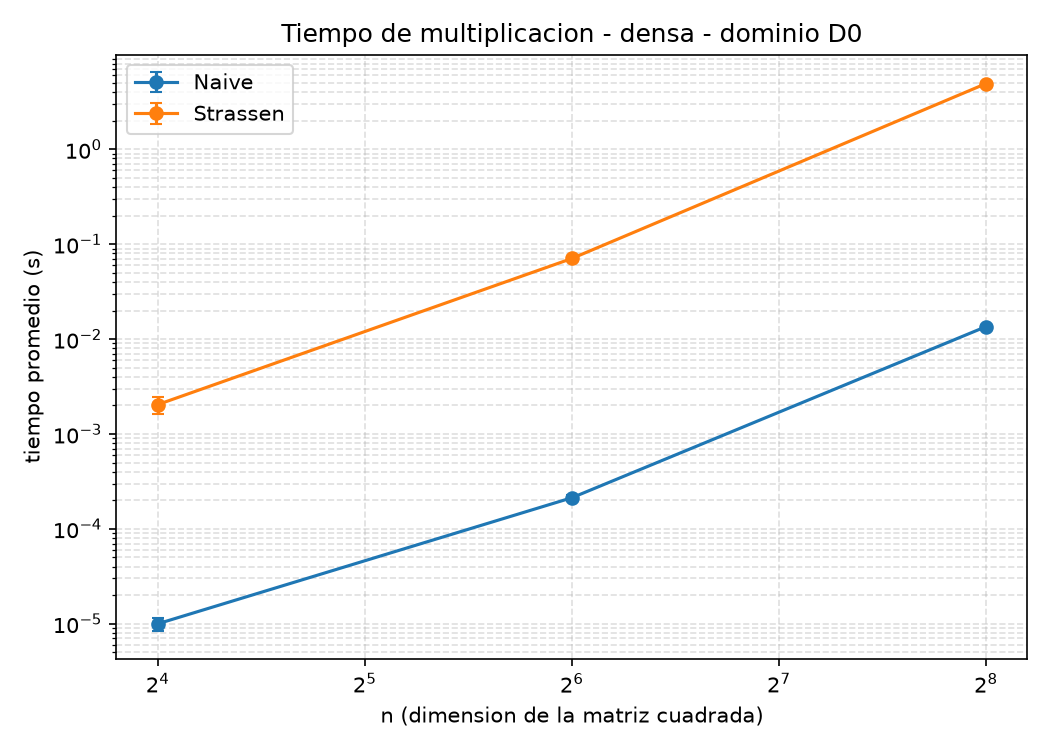
\includegraphics[width=0.7\textwidth]{../code/matrix_multiplication/data/plots/tiempo_densa_D0.png}
    \caption{Tiempo de multiplicación, matrices densas, dominio D0.}
    \label{fig:tiempo_matriz}
\end{figure}

Sorprendentemente, \textsc{Strassen} resultó entre 200 y 364 veces más
lento que \textsc{Naive} en todo el rango medido ($n=16$ a $n=256$),
pese a tener menor complejidad asintótica ($O(n^{\log_2 7}) \approx
O(n^{2.807})$ frente a $O(n^3)$) (los calculos fueron realizados extrayendo los valores de los archivos csv). Más aún, al comparar la tasa de
crecimiento entre $n=64$ y $n=256$ (un aumento de $4\times$ en $n$),
\textsc{Naive} creció $63.6\times$ --prácticamente idéntico a los
$64\times$ que predice $O(n^3)$--, mientras que \textsc{Strassen}
creció $69.7\times$, \textbf{superando} el $54.7\times$ que predice su
propia complejidad teórica $O(n^{2.807})$. Esto indica que el
comportamiento de \textsc{Strassen} en este rango no está dominado por
la cantidad de operaciones aritméticas (que sí sigue de cerca su cota
asintótica), sino por las instancias creadas en recursion, generando multiples vector<vector<int>>.

El uso de memoria (Figura~\ref{fig:memoria_matriz}) confirma este
diagnóstico: \textsc{Strassen} usa consistentemente entre 6.9x y 9.1x
más memoria que \textsc{Naive} para el mismo $n$, coherente con la
gran cantidad de matrices temporales que crea en cada nivel de
recursión. Además, la memoria fue idéntica (desviación estándar 0.0000
MB) entre los tipos densa/diagonal/dispersa para cada combinación
(algoritmo, $n$), lo cual es esperado dado que ninguna de las dos
implementaciones ajusta su estructura de datos según la dispersión de
la matriz.

\begin{figure}[h!]
    \centering
    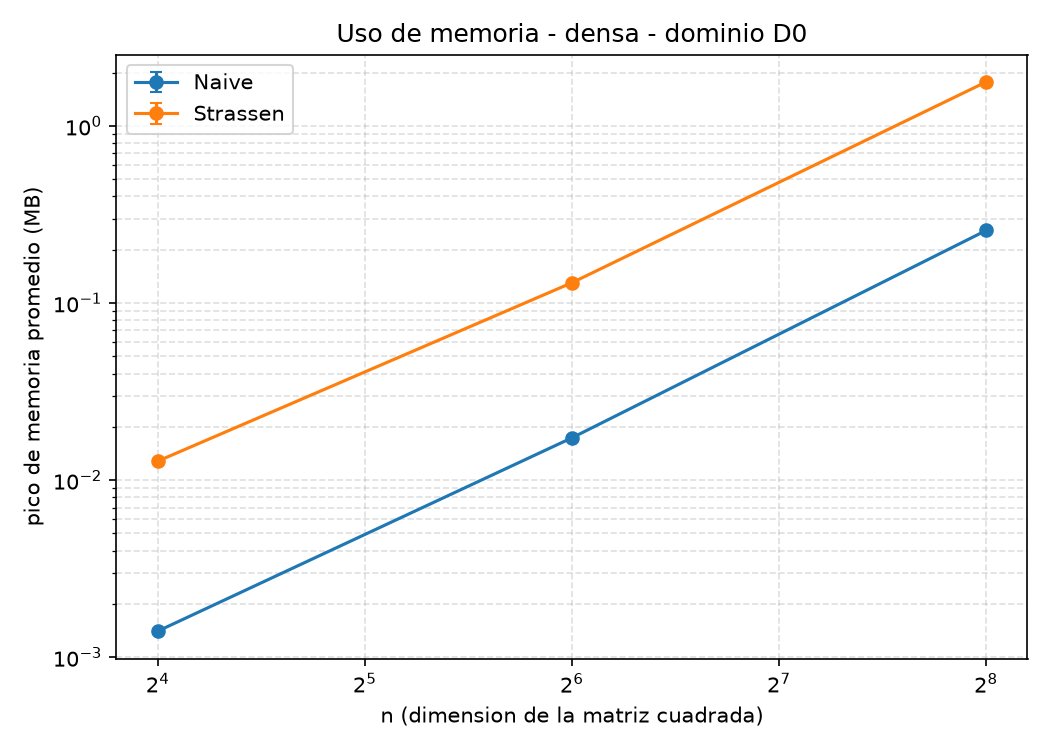
\includegraphics[width=0.7\textwidth]{../code/matrix_multiplication/data/plots/memoria_densa_D0.png}
    \caption{Uso de memoria, matrices densas, dominio D0.}
    \label{fig:memoria_matriz}
\end{figure}

Este resultado ilustra el objetivo central del experimento: la
notación asintótica describe el comportamiento cuando $n \to \infty$,
pero no garantiza mejor desempeño para los tamaños de entrada
efectivamente utilizados en la práctica, especialmente cuando la
implementación introduce overheads (aquí, de gestión de memoria) que
la notación no captura.

\subsection{Ordenamiento de arreglos}

Las Figuras~\ref{fig:tiempo_asc} y~\ref{fig:tiempo_ale} muestran el
tiempo de ordenamiento para $n=10^7$ en los casos ascendente y
aleatorio, comparando los dominios D1 (10 valores posibles, con
altísima tasa de repetición) y D7 ($10^7+1$ valores posibles, casi
todos distintos).

\begin{figure}[h!]
    \centering
    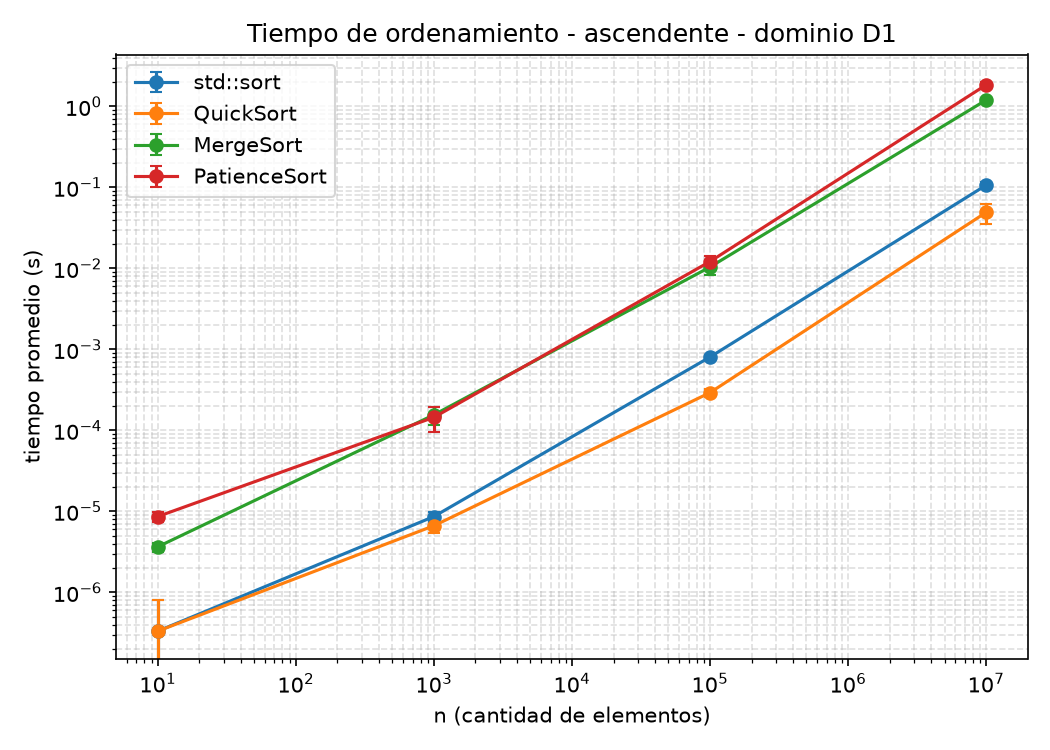
\includegraphics[width=0.48\textwidth]{../code/sorting/data/plots/tiempo_ascendente_D1.png}
    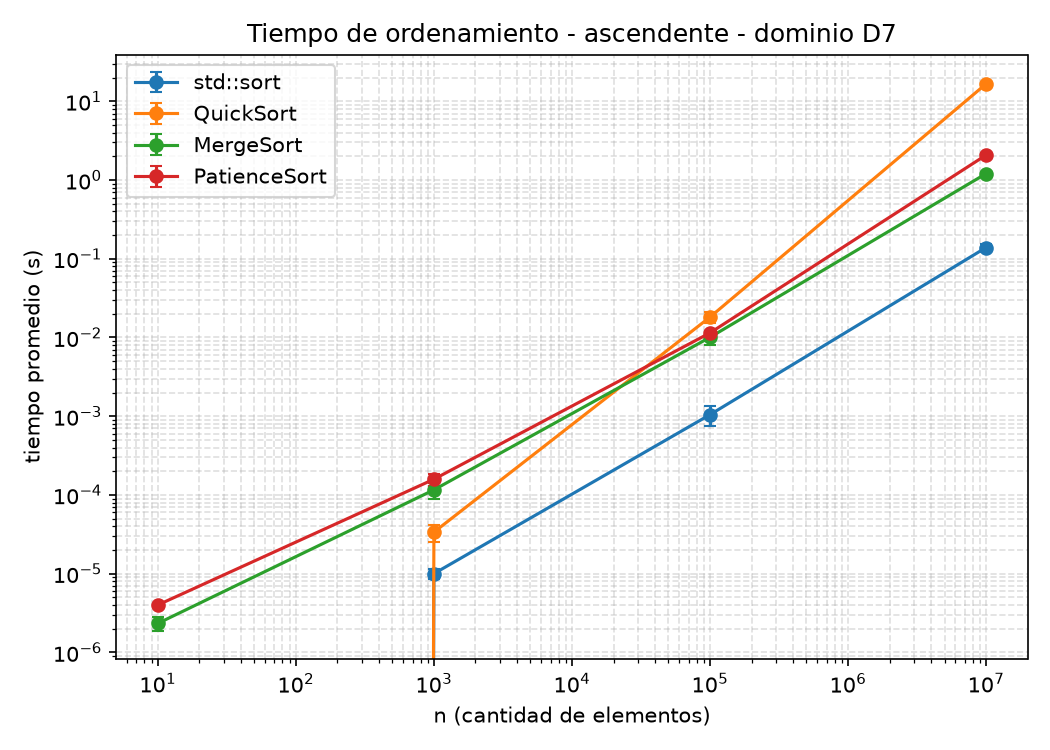
\includegraphics[width=0.48\textwidth]{../code/sorting/data/plots/tiempo_ascendente_D7.png}
    \caption{Tiempo de ordenamiento, caso ascendente, dominios D1 y D7.}
    \label{fig:tiempo_asc}
\end{figure}

\begin{figure}[h!]
    \centering
    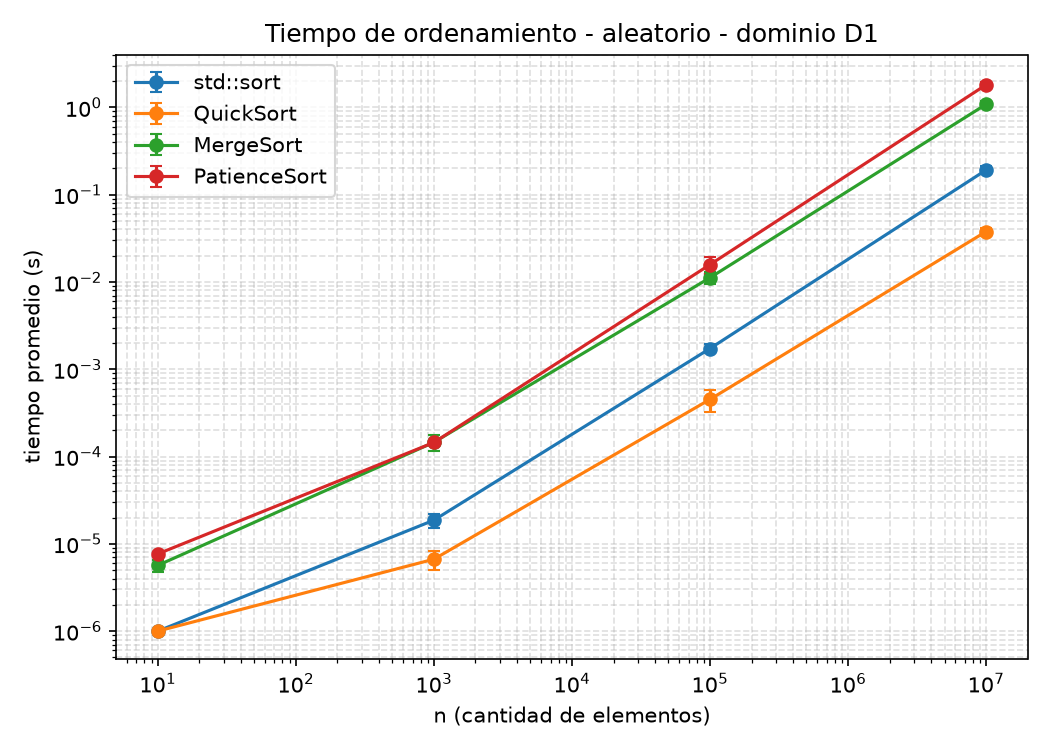
\includegraphics[width=0.48\textwidth]{../code/sorting/data/plots/tiempo_aleatorio_D1.png}
    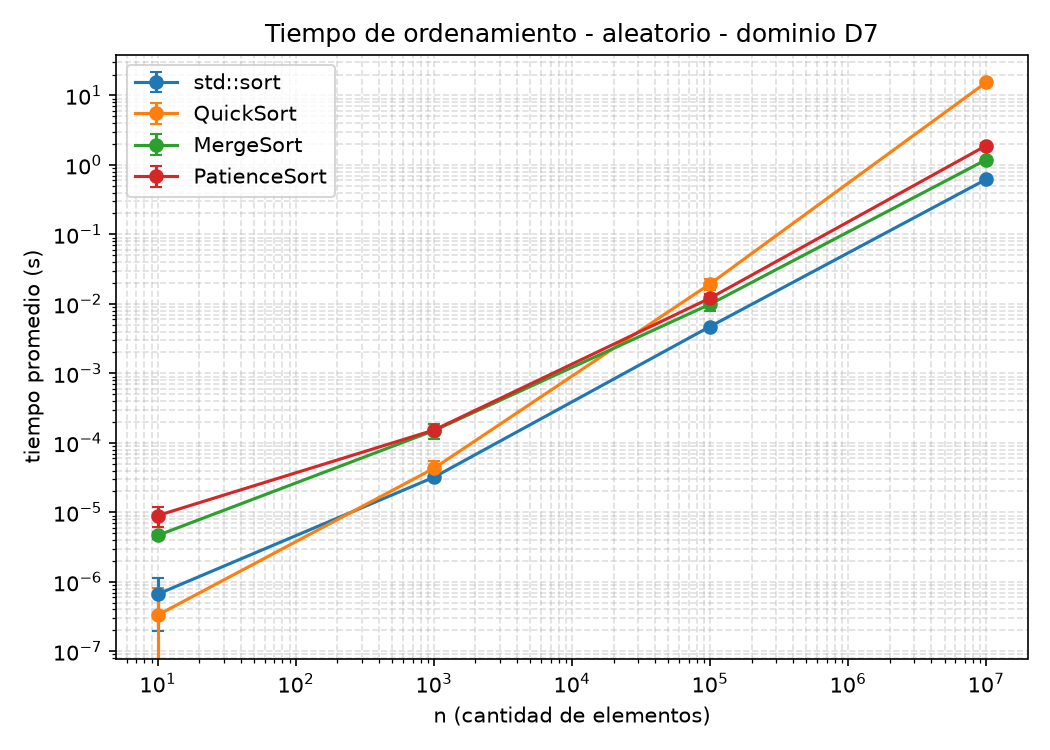
\includegraphics[width=0.48\textwidth]{../code/sorting/data/plots/tiempo_aleatorio_D7.png}
    \caption{Tiempo de ordenamiento, caso aleatorio, dominios D1 y D7.}
    \label{fig:tiempo_ale}
\end{figure}

\textsc{QuickSort} es, con diferencia, el caso más interesante. En
D1, su partición de 3 vías absorbe grandes bloques de elementos
iguales al pivote en cada llamada, lo que lo acerca a un
comportamiento casi lineal: a $n=10^7$ termina en apenas
$0.04$--$0.10$\,s en los tres tipos de entrada, superando incluso a
\texttt{std::sort}. En D7, en cambio, el comportamiento depende
fuertemente del orden de los datos: en el caso \textit{aleatorio}
toma $0.75$\,s (solo $7.4\times$ más que D1, la diferencia esperable
por la pérdida del beneficio de los duplicados), pero en los casos
\textit{ascendente} y \textit{descendente} explota a $14.4$\,s y
$10.3$\,s respectivamente ---$331\times$ y $265\times$ más lento que
su contraparte D1---, muy por encima del resto de los algoritmos.

Esto no es una falla del pivote fijo del \textsc{QuickSort} clásico
(que la mediana de tres ya evita), sino una variante del fenómeno
conocido en la literatura como \textit{"median-of-three killer"}
\cite{mcilroy1999}: la técnica de mediana de tres, al colocar el
pivote correcto en la última posición mediante intercambios directos,
puede desplazar el valor máximo del rango justo al centro de un
arreglo que sigue ordenado, generando particiones muy desbalanceadas
en niveles sucesivos de la recursión. El efecto solo se manifiesta
cuando los valores son casi todos distintos (D7); con alta repetición
(D1) la partición de 3 vías elimina la estructura ordenada antes de
que el desbalance se acumule, lo que explica por qué D1 nunca sufre
este problema sin importar el tipo de entrada.

\textsc{MergeSort} y \textsc{PatienceSort}, en cambio, muestran tiempos
consistentes entre tipos y dominios (variación menor a $2\times$ en
todos los casos), como corresponde a algoritmos cuya complejidad no
depende del orden ni de la repetición de los datos de entrada.

\begin{table}[h!]
\centering
\caption{Tiempo promedio de QuickSort a $n=10^7$ (segundos).}
\begin{tabular}{lcc}
\toprule
Tipo & D1 & D7 \\
\midrule
Ascendente  & 0.044 & 14.440 \\
Descendente & 0.039 & 10.296 \\
Aleatorio   & 0.101 & 0.754 \\
\bottomrule
\end{tabular}
\label{tab:quicksort_d1_d7}
\end{table}

Este resultado refuerza el mensaje central del experimento: una
optimización que en teoría debería blindar contra el peor caso
clásico (mediana de tres contra el pivote fijo) puede introducir, en
la práctica, una vulnerabilidad distinta y menos conocida, que solo
se manifiesta bajo condiciones específicas de los datos de entrada.